\documentclass[a4paper,12pt]{article}
\usepackage[left=2cm,right=2cm,top=2cm,bottom=2cm]{geometry} % Do ustawień marginesów
\usepackage{multicol} % Dla podziału na kolumny
\usepackage{ragged2e} % Dla justowania tekstu
\usepackage{graphicx} % Required for inserting images
\usepackage{float}
\usepackage{caption}
\usepackage{amsmath} % Math formulas
\usepackage{amssymb} % Symbols
\usepackage[svgnames]{xcolor}
\usepackage[colorlinks=true, urlcolor=blue, linkcolor=black, citecolor=orange]{hyperref} % Hyperlinks
\usepackage{polski} % Polish language
\usepackage[utf8]{inputenc} % Text encoding
\usepackage{enumitem} % Pakiet do elastycznego sterowania listami
\usepackage{indentfirst}
\usepackage{array}

\begin{document}

% Górna część strony
\noindent
\begin{minipage}{0.5\textwidth}
    \raggedright
    \textbf{Piotr Durniat} \\
    I rok, Fizyka \\
    Wtorek, 8:00-10:15 \\
    \vspace{0.5cm}
    \vspace{0.5cm}
\end{minipage}%
\begin{minipage}{0.5\textwidth}
    \raggedleft
    Data wykonania pomiarów: \\
    01.04.2025 \\
    \vspace{0.5cm} % Dodatkowa linia przerwy
    Prowadząca: \\
    dr Iwona Mróz
\end{minipage}

% Tytuł ćwiczenia
\vspace{2cm} % Odstęp
\begin{center}
    \LARGE \textbf{Ćwiczenie nr 15} \\[0.5cm]
    \Large \textbf{Drgania masy zawieszonej na sprężynie}
\end{center}

% Reszta treści
\vspace{1cm} % Kolejny odstęp
\noindent

\tableofcontents
\newpage

% ---------- WSTĘP TEORETYCZNY ----------
\section{Wstęp teoretyczny}

W doświadczeniu badamy ruch drgający masy zawieszonej na sprężynie. Podstawą teoretyczną jest prawo Hooke'a oraz równanie ruchu harmonicznego.

\subsection*{Prawo Hooke'a}
Prawo Hooke'a opisuje zależność siły sprężystości $F_s$ od wydłużenia sprężyny $\Delta x$:
\begin{equation}
    F_s = -k\Delta x
\end{equation}
gdzie $k$ jest współczynnikiem sprężystości sprężyny. Znak minus oznacza, że siła sprężystości działa przeciwnie do kierunku wychylenia.

\subsection*{Równanie ruchu harmonicznego}
Dla masy $m$ zawieszonej na sprężynie, zgodnie z II zasadą dynamiki Newtona:
\begin{equation}
    m\frac{d^2x}{dt^2} = -kx
\end{equation}

Rozwiązaniem tego równania jest funkcja:
\begin{equation}
    x(t) = A\sin(\omega t + \phi)
\end{equation}
gdzie:
\begin{itemize}
    \setlength{\itemsep}{0em}
    \item $A$ -- amplituda drgań
    \item $\omega = \sqrt{\frac{k}{m}}$ -- częstość kołowa drgań
    \item $\phi$ -- faza początkowa
\end{itemize}

\subsection*{Okres drgań}
Okres drgań $T$ masy zawieszonej na sprężynie wyraża się wzorem:
\begin{equation}
    \label{eq:okres}
    T = 2\pi\sqrt{\frac{m}{k}}
\end{equation}

Wzór \eqref{eq:okres} uwzględnia jedynie masę zawieszoną na sprężynie, jednakże w drganiach bierze udział również masa sprężyny. Uwzględniając ją należy dodać do masy ciężarka  $\frac{1}{3}$ masy sprężyny $m_{spr}$. Otrzymujemy w ten sposób wzór:

\begin{equation}
    \label{eq:okres_spr}
    T = 2\pi\sqrt{\frac{m + \frac{1}{3}m_{spr}}{k}}
\end{equation}

Z powyższego wzoru wynika zależność kwadratu okresu drgań od masy:
\begin{equation}
    \label{eq:okres_spr_2}
    T^2 = \frac{4\pi^2}{k}m + \frac{4\pi^2m_{spr}}{3k}
\end{equation}
gdzie $m_{spr}$ jest masą sprężyny.

\subsection*{Izochronizm drgań}
Teoretycznie, dla małych amplitud, okres drgań nie zależy od amplitudy. Jest to tzw. izochronizm drgań, który sprawdzamy w pierwszej części doświadczenia.

Niniejszy wstęp teoretyczny opracowano na podstawie podręcznika Ćwiczenia laboratoryjne z fizyki - rozdział 24 \cite{Drynski1976}.

% ---------- OPIS DOŚWIADCZENIA ----------
\section{Opis doświadczenia}

Celem doświadczenia jest zbadanie drgań masy zawieszonej na sprężynie poprzez realizację trzech zadań:

\subsection*{Badanie izochronizmu drgań}
\begin{itemize}
    \setlength{\itemsep}{0em}
    \item Używając masy 50 g, wykonano pomiary czasu 20 pełnych drgań dla amplitud od 1 do 10 cm
    \item Dla amplitudy 5 cm wykonano 5 powtórzeń pomiaru
    \item Celem było sprawdzenie, czy okres drgań zależy od amplitudy
\end{itemize}

\subsection*{Wyznaczanie współczynnika sprężystości $k$}
\begin{itemize}
    \setlength{\itemsep}{0em}
    \item Wykonano pomiary wydłużenia sprężyny dla mas od 10 do 60 g (co 10 g)
    \item Pomiary wykonano dwukrotnie: przy zwiększaniu i zmniejszaniu obciążenia
    \item Na podstawie wykresu zależności wydłużenia od siły sprawdzono zakres stosowalności prawa Hooke'a
\end{itemize}

\subsection*{Badanie zależności okresu drgań od masy}
\begin{itemize}
    \setlength{\itemsep}{0em}
    \item Zmierzono czas 10 pełnych drgań dla mas od 10 do 50 g (co 10 g)
    \item Wykonano dodatkowy pomiar dla masy nieznanej $m_x$
    \item Na podstawie zależności $T^2$ od $m$ wyznaczono masę nieznaną oraz parametry układu
\end{itemize}

Podczas wszystkich pomiarów położenia wykorzystano lusterko umieszczone obok metrówki, aby zapewnić prawidłowy odczyt poprzez pokrycie się wskaźnika sprężyny z jego odbiciem.


% ---------- OPRACOWANIE WYNIKÓW POMIARÓW ----------
\section{Opracowanie wyników pomiarów}

% ---------- TABELE ----------
\subsection{Tabele pomiarowe}

\begin{table}[H]
    \centering
    \begin{tabular}{|c|c|c|}
        \hline
        Nr & $A$ [cm] & $t(20 \text{ drgań})$ [s] \\
        \hline
        1  & 1 & 31,50 \\
        2  & 2 & 31,31 \\
        3  & 3 & 31,41 \\
        4  & 4 & 31,50 \\
        5  & 5 & 31,31 \\
        6  & 6 & 31,43 \\
        7  & 7 & 31,44 \\
        8  & 8 & 31,28 \\
        9  & 9 & 31,34 \\
        10 & 10 & 31,50 \\
        \hline
    \end{tabular}
    \caption{Zależność okresu drgań od amplitudy}
\end{table}

\begin{table}[H]
    \centering
    \begin{tabular}{|c|c|}
        \hline
        Nr & $t(20 \text{ drgań})$ [s] \\
        \hline
        1 & 31,44 \\
        2 & 31,16 \\
        3 & 31,28 \\
        4 & 31,34 \\
        5 & 31,66 \\
        \hline
    \end{tabular}
    \caption{Pomiar okresu dla $A = 5 \text{ cm}$}
    \label{tab:okres_5cm}
\end{table}

\begin{table}[H]
    \centering
    \begin{tabular}{|c|c|c|}
        \hline
        Nr & $m$ [g] & $x$ [cm] \\
        \hline
        1  & 10  & 21,0 \\
        2  & 20  & 28,2 \\
        3  & 30  & 35,4 \\
        4  & 40  & 42,6 \\
        5  & 50  & 50,0 \\
        6  & 60  & 57,1 \\
        \hline
        7  & 60  & 57,1 \\
        8  & 50  & 50,0 \\
        9  & 40  & 42,8 \\
        10 & 30  & 35,5 \\
        11 & 20  & 28,2 \\
        12 & 10  & 21,0 \\
        \hline
    \end{tabular}
    \caption{Zależność położenia szalki od masy}
\end{table}

\begin{table}[H]
    \centering
    \begin{tabular}{|c|c|c|}
        \hline
        $m$ [g] & $t(20 \text{ drgań})\,[\text{s}]$ & $t(10 \text{ drgań})\,[\text{s}]$ \\
        \hline
        10 & 25,41 & 12,81 \\
        20 & 26,13 & 13,94 \\
        30 & 29,53 & 14,81 \\
        40 & 31,47 & 15,59 \\
        50 & 33,06 & 16,60 \\
        60 & 34,72 & 17,84 \\
        $m_x$ & 33,22 & 14,91 \\
        \hline
    \end{tabular}
    \caption{Zależność okresu drgań od masy}
\end{table}

\subsection{1. Izochronizm drgań}

Okres drgań $T$ wyznaczono na podstawie zmierzonego czasu $t$ dla $n$ drgań, ze wzoru:
\[
    T = \frac{t}{n}
\]
gdzie:
\begin{itemize}
    \item $t$ -- zmierzony czas dla $n$ drgań,
    \item $n$ -- liczba drgań.
\end{itemize}

Na podstawie uzyskanych czasów obliczono okresy drgań sprężyny dla każdej amplitudy:

\begin{table}[H]
    \centering
    \begin{tabular}{|c|c|c|c|}
        \hline
        Nr & A [cm] & $t(20\,\text{drgań})$ [s] & $T$ [s] \\
        \hline
        1  & 1  & 31{,}50 & 1{,}575 \\
        2  & 2  & 31{,}31 & 1{,}5655 \\
        3  & 3  & 31{,}41 & 1{,}5705 \\
        4  & 4  & 31{,}50 & 1{,}575 \\
        5  & 5  & 31{,}31 & 1{,}5655 \\
        6  & 6  & 31{,}43 & 1{,}5715 \\
        7  & 7  & 31{,}44 & 1{,}572 \\
        8  & 8  & 31{,}28 & 1{,}564 \\
        9  & 9  & 31{,}34 & 1{,}567 \\
        10 & 10 & 31{,}50 & 1{,}575 \\
        \hline
    \end{tabular}
    \caption{Obliczone okresy drgań dla różnych amplitud}
\end{table}

Dla amplitudy $A = 5\,\text{cm}$ wykonano pięć pomiarów, na podstawie których obliczono wartości okresów:

\begin{table}[H]
    \centering
    \begin{tabular}{|c|c|c|}
        \hline
        Nr & $t(20\,\text{drgań})$ [s] & $T$ [s] \\
        \hline
        1 & 31{,}44 & 1{,}572 \\
        2 & 31{,}16 & 1{,}558 \\
        3 & 31{,}28 & 1{,}564 \\
        4 & 31{,}34 & 1{,}567 \\
        5 & 31{,}66 & 1{,}583 \\
        \hline
    \end{tabular}
    \caption{Pomiary okresu dla amplitudy $A = 5\,\text{cm}$}
\end{table}

Na podstawie powyższych danych wyznaczono średni okres:
\[
    T_{\text{śr}} = \frac{1{,}572 + 1{,}558 + 1{,}564 + 1{,}567 + 1{,}583}{5} = 1{,}569\,\text{s}
\]

Maksymalne odchylenie od średniej definiuje się jako:
\[
    \Delta T_{\text{max}} = \max\left(T_{\text{max}} - T_{\text{śr}},\ T_{\text{śr}} - T_{\text{min}}\right)
\]

Podstawiając wartości otrzymano:
\[
    \Delta T_{\text{max}} = \max(1{,}583 - 1{,}569,\ 1{,}569 - 1{,}558) = 0{,}014\,\text{s}
\]

Wyniki pomiarów okresu dla wszystkich amplitud mieszczą się w przedziale niepewności:
\[
    (T_{\text{śr}} - \Delta T_{\text{max}},\ T_{\text{śr}} + \Delta T_{\text{max}}) = (1{,}555,\ 1{,}583) \text{ s}
\]

% ---------- OBLICZENIA ----------
\subsection{2.  Zakres stosowalności prawa Hooke'a}


Dla szalki bez obciążenia położenie wynosi $x_0 = 13.6$ cm.
Na podstawie wyników obliczono wydłużenie $\Delta x_i$ jako różnicę między położeniem przy obciążeniu a położeniem początkowym:

\begin{equation}
    \label{eq:wydluzenie}
    \Delta x_i = x_i - x_0
\end{equation}

Następnie obliczono średnie wartości wydłużeń sprężyny \(x_i\) pod wpływem określonych obciążeń zgodnie ze wzorem:

\begin{equation*}
    \overline{\Delta x_i} = \frac{\Delta x_{i1} + \Delta x_{i2}}{2}
\end{equation*}

gdzie:
\begin{itemize}
    \setlength{\itemsep}{0em}
    \item \(\Delta x_{i1}\) -- wydłużenie szalki z masą \(m_i\) przy obciążeniu rosnącym,
    \item \(\Delta x_{i2}\) -- wydłużenie przy obciążeniu malejącym.
\end{itemize}

Wyniki obliczeń wydłużeń przedstawiono w tabeli \ref{tab:delta_x}.

\begin{table}[H]
    \centering
    \begin{tabular}{|c|c|c|}
        \hline
        $m$ [kg] & $\Delta x_1$ [m] & $\Delta x_2$ [m] \\
        \hline
        0,010 & 0,074 & 0,074 \\
        0,020 & 0,146 & 0,146 \\
        0,030 & 0,218 & 0,219 \\
        0,040 & 0,290 & 0,292 \\
        0,050 & 0,364 & 0,364 \\
        0,060 & 0,435 & 0,435 \\
        \hline
    \end{tabular}
    \caption{Wartości wydłużeń sprężyny}
    \label{tab:delta_x}
\end{table}

Ciężar $F$ został obliczony ze wzoru:

\begin{equation*}
    F = mg
\end{equation*}

gdzie:
\begin{itemize}
    \setlength{\itemsep}{0em}
    \item $m$ -- masa odważnika [kg],
    \item $g$ -- przyspieszenie ziemskie [m/s$^2$].
\end{itemize}

W obliczeniach przyjęto wartość przyspieszenia ziemskiego $g = 9,81$ m/s$^2$.
Wyniki obliczeń przedstawiono w tabeli \ref{tab:wydluzenia}.
Wykres zależności wydłużenia sprężyny od ciężaru przedstawiono na rysunku \ref{fig:zaleznosci}.

\begin{table}[H]
    \centering
    \begin{tabular}{|c|c|c|}
        \hline
        $m$ [kg] & $F$ [N] & $\overline{\Delta x}$ [m] \\
        \hline
        0,010 & 0,0981 & 0,074 \\
        0,020 & 0,1962 & 0,146 \\
        0,030 & 0,2943 & 0,2185 \\
        0,040 & 0,3924 & 0,291 \\
        0,050 & 0,4905 & 0,364 \\
        0,060 & 0,5886 & 0,435 \\
        \hline
    \end{tabular}
    \caption{Średnie wartości wydłużeń sprężyny}
    \label{tab:wydluzenia}
\end{table}

\subsubsection{Współczynnik sprężystości}

W celu wyznaczenia współczynnika sprężystości sprężyny zastosowano regresję liniową dla zależności wydłużenia $\Delta x$ od siły $F$ wykorzystując język Python i bibliotekę NumPy. Na podstawie równania regresji:

\begin{equation*}
    \Delta x = aF + b
\end{equation*}

gdzie:
\begin{itemize}
    \setlength{\itemsep}{0em}
    \item $a = \frac{1}{k}$ -- współczynnik kierunkowy prostej [m/N],
    \item $b$ -- wyraz wolny [m].
\end{itemize}

otrzymano następujące wartości:
\begin{itemize}
    \setlength{\itemsep}{0em}
    \item $a = 0,7373$ m/N,
    \item $b = 0,00160$ m.
\end{itemize}

Stąd współczynnik sprężystości wynosi:

\begin{equation*}
    k = \frac{1}{a} = \frac{1}{0{,}7373} \approx 1{,}356 \frac{\text{N}}{\text{m}}
\end{equation*}



\subsection{Analiza zależności kwadratu okresu od masy}

Poszukujemy zależności liniowej w postaci:
\[
    T^2 = a \cdot m + b
\]

\subsubsection*{Zestawienie wyników pomiarów:}
\begin{center}
    \begin{tabular}{|c|c|}
        \hline
        Masa $m$ [kg] & Kwadrat okresu $T^2$ [s$^2$] \\
        \hline
        0.028 & 1.6142 \\
        \hline
        0.038 & 1.7069 \\
        \hline
        0.048 & 2.1800 \\
        \hline
        0.058 & 2.4759 \\
        \hline
        0.068 & 2.7324 \\
        \hline
        0.078 & 3.0137 \\
        \hline
    \end{tabular}
\end{center}

\subsubsection*{Wielkości pomocnicze do obliczeń:}

\begin{align*}
    \text{Liczba pomiarów }n             & = 6        \\
    \text{Suma mas }\sum x_i             & = 0.318    \\
    \text{Suma }T^2\text{ }\sum y_i      & = 13.7229  \\
    \text{Suma kwadratów mas }\sum x_i^2 & = 0.018884 \\
    \text{Suma iloczynów }\sum x_i y_i   & = 0.76735  \\
\end{align*}

\subsubsection*{Wyznacznik układu równań $D$:}
\[
    D = n \sum x_i^2 - (\sum x_i)^2 = 6 \cdot 0.018884 - (0.318)^2 = 0.01218
\]

\subsubsection*{Parametry prostej regresji:}

Współczynnik kierunkowy \( a \):
\[
    a = \frac{n \sum x_i y_i - \sum x_i \sum y_i}{D} = \frac{4.6041 - 4.3659}{0.01218} \approx 29.63 \, \text{s}^2/\text{kg}
\]

Punkt przecięcia z osią $T^2$ \( b \):
\[
    b = \frac{\sum x_i^2 \cdot \sum y_i - \sum x_i \cdot \sum x_i y_i}{D} = \frac{0.018884 \cdot 13.7229 - 0.318 \cdot 0.76735}{0.01218} \approx 0.72 \ \text{s}^2
\]

Otrzymana zależność empiryczna:
\[
    T^2 = 29.63 \cdot m + 0,72
\]
Graficzna reprezentacja tej zależności znajduje się w sekcji z wykresami.

\subsection*{Teoretyczne wartości współczynników prostej}
Dysponując wartością współczynnika sprężystości: \[
    k = 1{,}356 \, \frac{\text{N}}{\text{m}}
\]
Możemy wyznaczyć teoretyczne wartości współczynników $A$ i $B$ w równaniu:
\[
    T^2 = A \cdot m + B
\]
zgodnie ze wzorami:
\[
    A = \frac{4\pi^2}{k}, \qquad B = \frac{4\pi^2 m_{spr}}{3k}
\]

Dane do obliczeń:
\begin{itemize}
    \item \( k = 1{,}356 \, \frac{N}{m} \)
    \item \( m_{spr} = 74 \, \text{g} = 0{,}074 \, \text{kg} \)
    \item \( \pi^2 \approx 9{,}8696 \)
\end{itemize}

Po podstawieniu otrzymujemy:
\[
    A = \frac{4\pi^2}{k}=\frac{4\cdot9,87}{1,356}= 29,12
\]
\[
    B = \frac{4\pi^2 m_{spr}}{3k}=\frac{4\cdot 9,87\cdot 0,074}{3\cdot1,356}=0,72
\]

\subsubsection*{Wyznaczenie masy nieznanej $m_x$}

Wykorzystując otrzymaną zależność empiryczną:
\[
    T^2 = 29{,}63 \cdot m + 0{,}72
\]
oraz zmierzoną wartość \( T^2 = 2{,}76 \), uwzględniając masę szalki \( m_s = 0{,}018\ \text{kg} \), możemy zapisać:
\[
    2{,}76 = 29{,}63 \cdot (m_x + 0{,}018) + 0{,}72
\]

Przekształcając kolejno:
\[
    2{,}04 = 29{,}63 \cdot (m_x + 0{,}018)
\]
\[
    m_x + 0{,}018 = \frac{2{,}04}{29{,}63} = 0{,}0689
\]
\[
    m_x = 0{,}0689 - 0{,}018 = 0{,}0509\ \text{kg} = 50{,}9\ \text{g}
\]





% ---------- NIEPEWNOŚCI ----------
\section{Ocena niepewności pomiaru}

\subsection{Niepewność czasu}

Niepewność typu B czasu obliczono ze wzoru:

\begin{equation*}
    u_B(t) = \frac{\Delta_d(t)}{\sqrt{3}}
\end{equation*}

Gdzie $\Delta_d(t) = 0,2$ to błąd eksperymentatora, stąd:

\begin{equation*}
    u_B(t) = \frac{0,2}{\sqrt{3}} \approx 0,12 \text{ s}
\end{equation*}

Niepewność typu A czasu wyznaczono na podstawie pięciu powtórzonych pomiarów dla amplitudy 5 cm (tabela \ref{tab:okres_5cm}), wykorzystując wzór \ref{eq:niepewnosc_A}.

\begin{equation} \label{eq:niepewnosc_A}
    u_A(t) = \sqrt{\frac{1}{n-1} \sum_{i=1}^{n} (t_i - \bar{t})^2}
\end{equation}

Podstawiając wartości do wzoru \ref{eq:niepewnosc_A} otrzymano:

\begin{equation*}
    u_A(t) = 0{,}19 \text{ s}
\end{equation*}

Niepewność złożoną czasu obliczono ze wzoru:

\begin{equation*}
    u_c(t) = \sqrt{u_A(t)^2 + u_B(t)^2}
\end{equation*}

Podstawiając wartości do wzoru otrzymano:

\begin{equation*}
    u_c(t) = \sqrt{0{,}19^2 + 0{,}12^2} \approx 0{,}22 \text{ s}
\end{equation*}





\subsection{Niepewność okresu}

Okres obliczono ze wzoru:

\begin{equation*}
    T = \frac{t}{N}
\end{equation*}

Gdzie $N$ to liczba drgań, stąd:

\begin{equation*}
    u_c(T) = \frac{u_c(t)}{N}
\end{equation*}

podstawiając wartość niepewności czasu otrzymano:

\begin{equation*}
    u_c(T) = \frac{0,22}{20} \approx 0,011 \text{ s}
\end{equation*}


\subsection{Niepewność położenia}

Niepewność maksymalna miarki wynosi $\Delta_d = 0,001$ m. Niepewność wydłużenia obliczono ze wzoru:

\begin{equation*}
    u_B(x) = \frac{\Delta_d x}{\sqrt{3}}
\end{equation*}

Po podstawieniu wartości otrzymano:

\begin{equation*}
    u_B(x) = \frac{0,001}{3} = 0,00058 \text{ m}
\end{equation*}

\subsection{Niepewność wydłużenia}

Niepewność wydłużenia obliczono z prawa przenoszenia niepewności dla wzoru \ref{eq:wydluzenie}:

\begin{align*}
    u_c(\Delta x) & = \sqrt{\left(\frac{\partial \Delta x}{\partial x}\right)^2 u^2(x) + \left(\frac{\partial \Delta x}{\partial x_0}\right)^2 u^2(x_0)} \\
                  & = \sqrt{(1)^2 u^2(x) + (-1)^2 u^2(x_0)}                                                                                              \\
                  & = \sqrt{2} u_B(x)
\end{align*}

Stąd niepewność pojedynczego pomiaru wydłużenia:

\begin{equation*}
    u_c(\Delta x) = \sqrt{2} \cdot 0,00058 \approx 0,00082 \text{ m}
\end{equation*}

\subsection{Niepewność średniego wydłużenia}

\subsection*{Niepewność złożona średniego wydłużenia}

Dla średniego wydłużenia:
\begin{equation*}
    \overline{\Delta x_i} = \frac{\Delta x_{i1} + \Delta x_{i2}}{2}
\end{equation*}

niepewność złożoną możemy wyznaczyć korzystając z prawa propagacji niepewności:

\begin{align*}
    u_c(\overline{\Delta x_i}) & = \sqrt{\left(\frac{\partial \overline{\Delta x_i}}{\partial \Delta x_{i1}}\right)^2 u^2(\Delta x_{i1}) + \left(\frac{\partial \overline{\Delta x_i}}{\partial \Delta x_{i2}}\right)^2 u^2(\Delta x_{i2})} \\
                               & = \sqrt{\left(\frac{1}{2}\right)^2 u^2(\Delta x) + \left(\frac{1}{2}\right)^2 u^2(\Delta x)}                                                                                                               \\
                               & = \sqrt{\frac{2}{4} u^2(\Delta x)} = \frac{u(\Delta x)}{\sqrt{2}}
\end{align*}

Podstawiając wartość niepewności pojedynczego pomiaru wydłużenia otrzymano:

\begin{equation*}
    u_c(\overline{\Delta x_i}) = \frac{0,00082}{\sqrt{2}} \approx 0,00058 \text{ m}
\end{equation*}


\subsection{Współczynnik sprężystości}

Niepewności współczynników regresji liniowej dla zależności $x = a F + b$ obliczono na podstawie następujących wzorów:

\[
    s_y = \sqrt{\frac{\sum_{i=1}^{n} (y_i - \hat{y}_i)^2}{n-2}}
\]

\[
    u(k) = s_y \sqrt{\frac{n}{n \sum x_i^2 - \left( \sum x_i \right)^2}}
\]

\[
    u(b) = s_y \sqrt{\frac{\sum x_i^2}{n \sum x_i^2 - \left( \sum x_i \right)^2}}
\]

gdzie:

\begin{itemize}
    \setlength{\itemsep}{0em}
    \item $s_y$ -- odchylenie standardowe reszt,
    \item $u(a)$ -- niepewność standardowa współczynnika kierunkowego prostej regresji,
    \item $u(b)$ -- niepewność standardowa wyrazu wolnego prostej regresji,
    \item $n$ -- liczba punktów pomiarowych,
    \item $x_i$ -- wartości zmiennej niezależnej (siła $F$),
    \item $y_i$ -- wartości zmierzone (wydłużenie $\Delta x$),
    \item $\hat{y}_i$ -- wartości przewidywane przez model regresji,
\end{itemize}

Obliczone wartości niepewności dla współczynników prostej regresji wynoszą:

\begin{itemize}
    \setlength{\itemsep}{0em}
    \item $u(a) = 0,0012\,\frac{\text{m}}{\text{N}}$
    \item $u(b) = 0,00046\,\text{m}$
\end{itemize}

Współczynnik sprężystości wyraża się wzorem:

\begin{equation*}
    k = \frac{1}{a}
\end{equation*}

Stąd niepewność współczynnika sprężystości wynosi:

\begin{equation*}
    u(k) =  \frac{1}{a^2} \cdot u(a)
\end{equation*}

Podstawiając wartość niepewności współczynnika $a$ otrzymano:

\begin{equation*}
    u(k) =  \frac{1}{0{,}7373^2} \cdot 0,0012 \approx 0,0022 \frac{\text{m}}{\text{N}}
\end{equation*}



\subsection{Niepewności współczynników A i B zależności $T^2 = Am + B$}

Niepewności współczynników $A$ i $B$ zależności $T^2 = Am + B$ obliczono na podstawie następujących wzorów:

\[
    s_y = \sqrt{\frac{\sum_{i=1}^{n} (y_i - \hat{y}_i)^2}{n-2}}
\]

\[
    u(A) = s_y \sqrt{\frac{n}{n \sum m_i^2 - \left( \sum m_i \right)^2}}
\]

\[
    u(B) = s_y \sqrt{\frac{\sum m_i^2}{n \sum m_i^2 - \left( \sum m_i \right)^2}}
\]

gdzie:
\begin{itemize}
    \setlength{\itemsep}{0em}
    \item $s_y$ -- odchylenie standardowe reszt,
    \item $u(A)$ -- niepewność standardowa współczynnika kierunkowego prostej regresji,
    \item $u(B)$ -- niepewność standardowa wyrazu wolnego prostej regresji,
    \item $n$ -- liczba punktów pomiarowych,
    \item $m_i$ -- wartości mas efektywnych,
    \item $y_i$ -- wartości zmierzone ($T^2$),
    \item $\hat{y}_i$ -- wartości przewidywane przez model regresji.
\end{itemize}

Obliczone wartości niepewności dla współczynników prostej regresji wynoszą:

\begin{itemize}
    \setlength{\itemsep}{0em}
    \item $u(A) = 1{,}54\,\frac{\text{s}^2}{\text{kg}}$
    \item $u(B) = 0{,}12\,\text{s}^2$
\end{itemize}

\subsection{Niepewności współczynników A i B z wzorów}
Na podstawie wzoru \ref{eq:okres_spr_2} współczynniki $A$ i $B$ wyrażają się następującymi zależnościami:

\begin{equation*}
    A = \frac{4\pi^2}{k}
\end{equation*}

\begin{equation*}
    B = \frac{4\pi^2m_{spr}}{3k}
\end{equation*}



Korzystając ze wzoru na niepewność złożoną:
\begin{equation*}
    u_c(E) = \sqrt{\sum_{k=1}^{K} \left( \frac{\partial E}{\partial x_k} \right)^2 u^2(x_k)}
\end{equation*}

Dla współczynnika $A$ mamy tylko jedną zmienną (k), więc:
\begin{equation*}
    u_c(A) = \sqrt{\left(\frac{\partial A}{\partial k}\right)^2 u^2(k)}
\end{equation*}

Po podstawieniu pochodnej:
\begin{equation*}
    u_c(A) = \sqrt{\left(-\frac{4\pi^2}{k^2}\right)^2 u^2(k)}
\end{equation*}

Ostatecznie:
\begin{equation*}
    u_c(A) = \frac{4\pi^2}{k^2} u(k)
\end{equation*}

Podstawiając wartości:

\begin{equation*}
    u_c(A) = \frac{4\pi^2}{1.356^2} \cdot 0,0022 \approx 0,048 \frac{\text{s}^2}{\text{kg}}
\end{equation*}

Dla współczynnika $B$ mamy dwie zmienne (k i $m_{spr}$), lecz ze względu na brak informacji o niepewności masy sprężyny $u(m_{spr})$, ograniczymy się do obliczenia niepewności względem zmiennej k:

\begin{equation*}
    u_c(B) = \sqrt{\left(\frac{\partial B}{\partial k}\right)^2 u^2(k)}
\end{equation*}

Po podstawieniu pochodnej cząstkowej:
\begin{equation*}
    u_c(B) = \sqrt{\left(-\frac{4\pi^2m_{spr}}{3k^2}\right)^2 u^2(k)}
\end{equation*}

Ostatecznie:
\begin{equation*}
    u_c(B) = \frac{4\pi^2m_{spr}}{3k^2} u(k)
\end{equation*}


Podstawiając wartości:

\begin{equation*}
    u_c(B) = \frac{4 \cdot \pi^2 \cdot 0.074}{3 \cdot 1.356^2} \cdot 0.0022 \approx 0.0012 \text{s}^2
\end{equation*}



% ---------- WNIOSKI ----------
\section{Wnioski}

Wyniki eksperymentu wykazały, że w badanym zakresie amplitud (od 1 do 10 cm) okres drgań pozostaje stały w granicach błędu pomiarowego. Świadczy o tym fakt, że wszystkie wyznaczone wartości okresów znajdują się wewnątrz przedziału niepewności, który został określony na podstawie serii pięciu pomiarów wykonanych dla amplitudy 5 cm. Zaobserwowana niezależność okresu od amplitudy potwierdza występowanie zjawiska izochronizmu, które jest przewidywane przez teorię ruchu harmonicznego przy małych wychyleniach.

Na podstawie wyników pomiarów wyznaczono współczynnik sprężystości sprężyny $k = 0{,}7373 \frac{\text{m}}{\text{N}}$, $u(k)= 0{,}0022 \frac{\text{m}}{\text{N}}$ oraz wyraz wolny $b = 0{,}00160 \text{m}$, $u(b)= 0{,}00046 \text{m}$, który jest bliski zeru. Wykonane pomiary potwierdziły prawo Hooke'a w zakresie od 10 g do 60 g.


Otrzymane empirycznie współczynniki prostej regresji ($a = 29,63$ s²/kg, $b = 0,72$ s²) są bardzo zbliżone do wartości przewidzianych teoretycznie ($A = 29,12$ s²/kg, $B = 0,72$ s²). Wyraz wolny $b = 0,72$ s² odpowiada teoretycznej wartości wynikającej z uwzględnienia masy sprężyny, co potwierdza słuszność korekty $\frac{1}{3}m_{spr}$ w równaniu okresu drgań.

Wykorzystując otrzymaną zależność empiryczną, udało się wyznaczyć nieznaną masę $m_x = 50,9$ g.

% ---------- WYKRESY ----------
\section{Wykresy}

\begin{figure}[H]
    \centering
    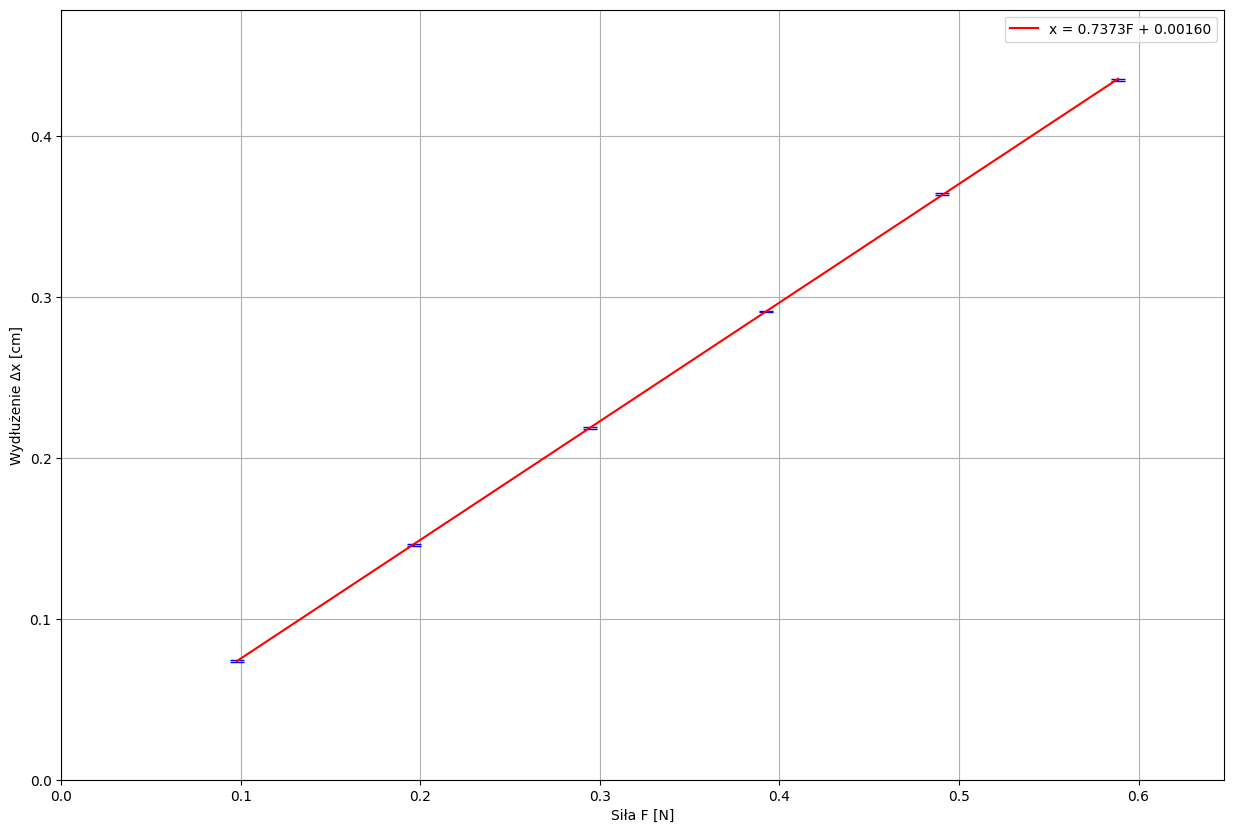
\includegraphics[width=1.2\linewidth,angle=90]{2-x(F).png}
    \caption{Zależność wydłużenia sprężyny od ciężaru (źródło: opracowanie własne).}
    \label{fig:zaleznosci}
\end{figure}

\begin{figure}[H]
    \centering
    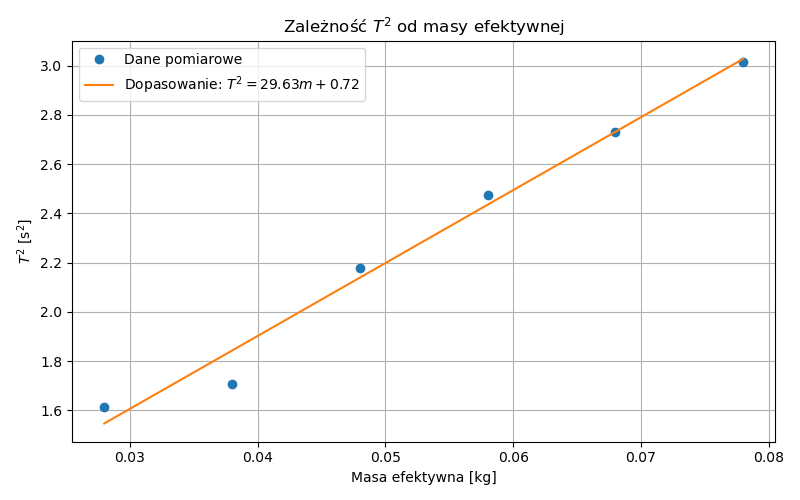
\includegraphics[width=1.2\linewidth,angle=90]{wykres_masy_efektywnej.png}
    \caption{Zależność wydłużenia sprężyny od ciężaru (źródło: opracowanie własne).}
    \label{fig:zaleznosci2}
\end{figure}




\bibliographystyle{plain}
\bibliography{bibliography}

\end{document}


